%-----------------------
% Title page
%-----------------------
\begin{titlepage}
  \centering

  \textsc{ELEC4630 Assignment 1}\\
  \vspace{9cm}

  \rule{\linewidth}{0.5pt}\\

  \vspace{1em}
  \LARGE\textsc{Question 3}\\
  \vspace{1em}

  \LARGE\uppercase{\textbf{{Hough Transforms}}}\\

  \rule{\linewidth}{2pt}\\

  \vfill

  \normalsize{Deren Teo (4528554)}
  \vspace{1cm}

\end{titlepage}

%-----------------------
% Report body
%-----------------------
\section{Introduction}

The Hough transform is a technique that can be used to detect any shape in an image, as long as the shape can be represented in mathematical form \cite{opencv_hlt}. This report presents a method of using the Hough line and circle transforms to identify various features in an image of Mr Bean and his car. The features of interest are the egde of the road, Mr Bean's broomstick and the wheel hubs of Mr Bean's car.

\section{Background Theory}

\subsection{Hough Line Transform}

\textit{(Please refer to Question 2 submission.)}

\subsection{Hough Circle Transform}

\subsection{Morphological Transformations}

\subsection{Canny Edge Detection}

\subsection{Contours}

\section{Methodology}

The presented solution is composed of three distinct sub-solutions, one for each of the desired features. The solutions are chained in sequence to produce the desired result.

First, for detecting the road edge:
\begin{enumerate}
  \item The image is converted to HSV and the saturation channel is extracted, which contrasts the road well against the grass.

  \item The image is binarized using an experimentally tuned threshold of 100. This separates the road from the rest of the background.

  \item The binarized image is morphologically closed using a very large kernel (121 x 121) to remove all detail except for the road edge border, which is possible because the road edge is the largest and most clearly defined detail in the binarized image.

  \item Canny edge detection is performed to define the road edge for the Hough line transform.

  \item The Hough line transform is then applied with an experimentally tuned threshold of 125 to identify the road edge. This threshold effectively filters out all noise.

  \item Using the method described in the Question 2 methodology, an equation for the road edge line is defined. The start and end points of each section of the road edge are not yet determined.

  \item To determine the start and end points of each road section, contour detection is performed on the morphologically closed image. This finds the position and size of each road section.

  \item Finally, the position and size of each road section are used to determine the start and end points of the road edge.

\end{enumerate}

Then, for detecting Mr Bean's broomstick:
\begin{enumerate}
  \item The image is converted to HSV and the saturation channel is extracted, which contrasts the broomstick fairly well against the grass.

  \item The image is binarized using an experimentally tuned threshold of 150. This separates the broomstick from most of the background as best as possible but produces a very noisy image.

  \item The morphological tophat transform is applied using a vertical kernel to black out large white sections without erasing the broomstick. This primarily removes Mr Bean himself and the car, leaving the broomstick as the largest remaining white object.

  \item The image is morphologically opened to remove some of the noise before applying the Hough line transform. A vertical kernel is again necessary to avoid erasing the broomstick, but results in the remaining noise being thin vertical lines.

  \item The Hough line transform is applied with a threshold tuned to ignore the remaining noise. If the morphological transforms were successful, then the broomstick should be the only detected line.

  \item Using the method described in the Question 2 methodology, the equation for the broomstick line is derived. However, the extents of the line are not yet known.

  \item To detect the extents of the line, contour detection is performed and the contours are sorted by size. The position and size of the largest contour are assumed to represent the broomstick.

  \item Using the position and size of the broomstick contour, the extents of the broomstick line can be determined.

\end{enumerate}

And finally, for detecting the wheel hubs of Mr Bean's car:
\begin{enumerate}
  \item The image is converted to grayscale and binarized using an experimentally tuned threshold of 50. This contrasts the wheel hubs strongly against the tires.

  \item The image is morphologically closed to remove noise, then contour detection is performed to identify circular contours.

  \item The contours are filtered by area to leave only wheel-sized contours. The wheels in the image are approximately 3000 sq. pixels, and the contours are filtered to between 2500 and 3500 sq. pixels.

  \item The contours are further filtered by aspect ratio, which is sufficient to distinguish the wheel hubs. The aspect ratios between 0.8 and 1.2 are kept.

  \item A bounding rectangle is used to find the size and shape of the remaining contours, which is used to define circles of the respective position and radius. Where the aspect ratio is not 1, the circle diameter is taken as the average of the bounding rectangle width and height.

\end{enumerate}

\section{Results}

Figure \ref{fig:q3results} presents the image of Mr Bean overlayed with red lines demarcating the identified features: the edge of the road, Mr Bean's broomstick, and the wheel hubs of Mr Bean's car.

\begin{figure}[ht]
  \centering
  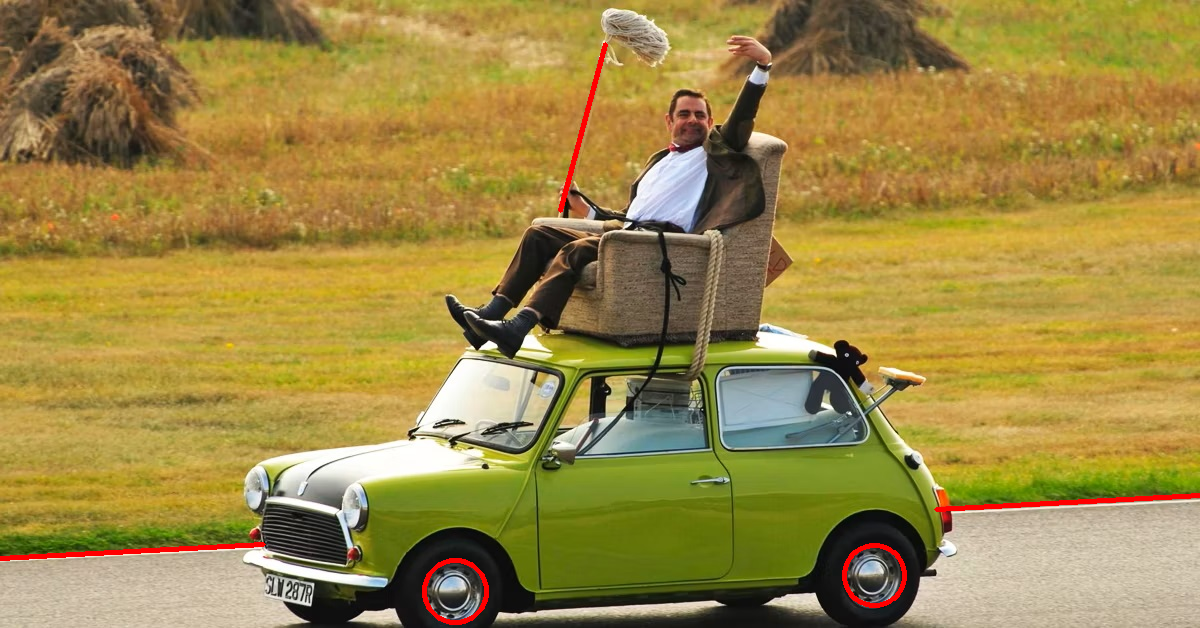
\includegraphics[width=0.6\textwidth]{images/q3_results.png}
  \caption{Features detected using contour detection and Hough transforms.}
  \label{fig:q3results}
\end{figure}

\newpage
\section{Discussion}

This report has presented a method of detecting several features in an image of Mr Bean and his car. The features of interest are: the road edge, Mr Bean's broomstick and the wheel hubs of Mr Bean's car. The method succesfully identifies all features, as evident in Figure \ref{fig:q3results}.

There are, however, certain caveats to the method which warrant further discussion.

Firstly, in detecting the road edge, the binarized image is morphologically closed using a very large kernel to remove all details except the road edge. This assumes the road edge is the most significant feature in the image, and will therefore remain after all other details are erased. If this is not true, for example if the car is near either side of the frame, the edge may not be properly detected. Furthermore, contour detection is used to identify the road sections in the closed image, which allows any number of road sections to be detected, anywhere in the image. However, it also assumes the only features remaining in the closed image are sections of the road. If this is untrue, road edges will be incorrectly identified.

Secondly, in detecting the broomstick, a manual vertical offset is implemented to account for the solution slightly misidentifying the position of the broomstick. The Hough line transform successfully identifies the broomstick line; however, when performing contour detection to identify the broomstick extent, the solution includes part of the chair and excludes the top of the broomstick. This is due to the extensive morphological operations performed to reduce noise disturbing the broomstick endpoints.

Finally, in detecting the wheel hubs, the Hough circle transform is not used. In spite of the aim of the question, it was found that pure contour detection provided a faster, simpler and more robust method of wheel detection than the Hough circle transform. The predominant reason is that the Hough circle transform requires the size of the wheels to be known. This necessitates a contour detection to identify circular shapes and provide their sizes. Yet, having already identified the circular shapes, there is no further need to apply the Hough circle transform.

\section{Conclusion}

In summary, this report presents a successful solution to the problem of identifying several features in an image of Mr Bean. The solution successfully identifies visible sections of road edge, Mr Bean's broomstick, and the wheel hubs of Mr Bean's car. However, shortcomings with the solution are present and discussed, largely surrounding the unknown level of robustness required of the solution given a sample size of one image.
